% ========================================
%	Header einbinden
% ========================================

\documentclass[bibtotoc,titlepage]{scrartcl}

% Deutsche Spracheinstellungen
\usepackage[ngerman,german]{babel, varioref}
\usepackage[T1]{fontenc}
\usepackage[utf8]{inputenc}

%\usepackage{marvosym}

\usepackage{amsfonts}
\usepackage{amssymb}
\usepackage{amsmath}
\usepackage{amscd}
\usepackage{amstext}

\usepackage{longtable}

%\usepackage{bibgerm}

\usepackage{footnpag}

\usepackage{ifthen}                 %%% package for conditionals in TeX
\usepackage[amssymb]{SIunits}
%Für textumflossene Bilder und Tablellen
%\usepackage{floatflt} - veraltet

%Für Testzwecke aktivieren, zeigt labels und refs im Text an.
%\usepackage{showkeys}

% Abstand zwischen zwei Absätzen nach DIN (1,5 Zeilen)
% \setlength{\parskip}{1.5ex plus0.5ex minus0.5ex}

% Einrückung am Anfang eines neuen Absatzes nach DIN (keine)
%\setlength{\parindent}{0pt}

% Ränder definieren
% \setlength{\oddsidemargin}{0.3cm}
% \setlength{\textwidth}{15.6cm}

% bessere Bildunterschriften
%\usepackage[center]{caption2}


% Problemlösungen beim Umgang mit Gleitumgebungen
\usepackage{float}

% Nummeriert bis zur Strukturstufe 3 (also <section>, <subsection> und <subsubsection>)
%\setcounter{secnumdepth}{3}

% Führt das Inhaltsverzeichnis bis zur Strukturstufe 3
%\setcounter{tocdepth}{3}
\usepackage[version=3]{mhchem}
	\mhchemoptions{minus-sidebearing-left=0.06em, minus-sidebearing-right=0.11em}
\usepackage{exscale}

\newenvironment{dsm} {\begin{displaymath}} {\end{displaymath}}
\newenvironment{vars} {\begin{center}\scriptsize} {\normalsize \end{center}}


\newcommand {\en} {\varepsilon_0}               % Epsilon-Null aus der Elektrodynamik
\newcommand {\lap} {\; \mathbf{\Delta}}         % Laplace-Operator
\newcommand {\R} { \mathbb{R} }                 % Menge der reellen Zahlen
\newcommand {\e} { \ \mathbf{e} }               % Eulersche Zahl
\renewcommand {\i} { \mathbf{i} }               % komplexe Zahl i
\newcommand {\N} { \mathbb{N} }                 % Menge der nat. Zahlen
\newcommand {\C} { \mathbb{C} }                 % Menge der kompl. Zahlen
\newcommand {\Z} { \mathbb{Z} }                 % Menge der kompl. Zahlen
\newcommand {\limi}[1]{\lim_{#1 \rightarrow \infty}} % Limes unendlich
\newcommand {\sumi}[1]{\sum_{#1=0}^\infty}
\newcommand {\rot} {\; \mathrm{rot} \,}         % Rotation
\newcommand {\grad} {\; \mathrm{grad} \,}       % Gradient
\newcommand {\dive} {\; \mathrm{div} \,}        % Divergenz
\newcommand {\dx} {\; \mathrm{d} }              % Differential d
\newcommand {\cotanh} {\; \mathrm{cotanh} \,}   %Cotangenshyperbolicus
\newcommand {\asinh} {\; \mathrm{areasinh} \,}  %Area-Sinus-Hyp.
\newcommand {\acosh} {\; \mathrm{areacosh} \,}  %Area-Cosinus-H.
\newcommand {\atanh} {\; \mathrm{areatanh} \,}  %Area Tangens-H.
\newcommand {\acoth} {\; \mathrm{areacoth} \,}  % Area-cotangens
\newcommand {\Sp} {\; \mathrm{Sp} \,}
\newcommand {\mbe} {\stackrel{\text{!}}{=}}     %Must Be Equal
\newcommand{\qed} { \hfill $\square$\\}
\renewcommand{\i} {\imath}
\def\captionsngerman{\def\figurename{\textbf{Abb.}}}

%%%%%%%%%%%%%%%%%%%%%%%%%%%%%%%%%%%%%%%%%%%%%%%%%%%%%%%%%%%%%%%%%%%%%%%%%%%%
% SWITCH FOR PDFLATEX or LATEX
%%%%%%%%%%%%%%%%%%%%%%%%%%%%%%%%%%%%%%%%%%%%%%%%%%%%%%%%%%%%%%%%%%%%%%%%%%%%
%%%
\ifx\pdfoutput\undefined %%%%%%%%%%%%%%%%%%%%%%%%%%%%%%%%%%%%%%%%% LATEX %%%
%%%
\usepackage[dvips]{graphicx}       %%% graphics for dvips
\DeclareGraphicsExtensions{.eps,.ps}   %%% standard extension for included graphics
\usepackage[ps2pdf]{thumbpdf}      %%% thumbnails for ps2pdf
\usepackage[ps2pdf,                %%% hyper-references for ps2pdf
bookmarks=true,%                   %%% generate bookmarks ...
bookmarksnumbered=true,%           %%% ... with numbers
hypertexnames=false,%              %%% needed for correct links to figures !!!
breaklinks=true,%                  %%% breaks lines, but links are very small
linkbordercolor={0 0 1},%          %%% blue frames around links
pdfborder={0 0 112.0}]{hyperref}%  %%% border-width of frames
%                                      will be multiplied with 0.009 by ps2pdf
%
\hypersetup{ pdfauthor   = {Hannes Franke; Julius Tilly},
pdftitle    = {V301 Innenwiderstand und Leistungsanpassung}, pdfsubject  = {Protokoll FP}, pdfkeywords = {V301, Innenwiderstand, Leistungsanpassung},
pdfcreator  = {LaTeX with hyperref package}, pdfproducer = {dvips
+ ps2pdf} }
%%%
\else %%%%%%%%%%%%%%%%%%%%%%%%%%%%%%%%%%%%%%%%%%%%%%%%%%%%%%%%%% PDFLATEX %%%
%%%
\usepackage[pdftex]{graphicx}      %%% graphics for pdfLaTeX
\DeclareGraphicsExtensions{.pdf}   %%% standard extension for included graphics
\usepackage[pdftex]{thumbpdf}      %%% thumbnails for pdflatex
\usepackage[pdftex,                %%% hyper-references for pdflatex
bookmarks=true,%                   %%% generate bookmarks ...
bookmarksnumbered=true,%           %%% ... with numbers
hypertexnames=false,%              %%% needed for correct links to figures !!!
breaklinks=true,%                  %%% break links if exceeding a single line
linkbordercolor={0 0 1},
linktocpage]{hyperref} %%% blue frames around links
%                                  %%% pdfborder={0 0 1} is the default
\hypersetup{
pdftitle    = {V301 Innenwiderstand und Leistungsanpassung}, 
pdfsubject  = {Protokoll AP}, 
pdfkeywords = {V301, Innenwiderstand, Leistungsanpassung},
pdfsubject  = {Protokoll AP},
pdfkeywords = {V301, Innenwiderstand, Leistungsanpassung}}
%                                  %%% pdfcreator, pdfproducer,
%                                      and CreationDate are automatically set
%                                      by pdflatex !!!
\pdfadjustspacing=1                %%% force LaTeX-like character spacing
\usepackage{epstopdf}
%
\fi %%%%%%%%%%%%%%%%%%%%%%%%%%%%%%%%%%%%%%%%%%%%%%%%%%% END OF CONDITION %%%
%%%%%%%%%%%%%%%%%%%%%%%%%%%%%%%%%%%%%%%%%%%%%%%%%%%%%%%%%%%%%%%%%%%%%%%%%%%%
% seitliche Tabellen und Abbildungen
%\usepackage{rotating}
\usepackage{ae}
\usepackage{
  array,
  booktabs,
  dcolumn
}
\makeatletter 
  \renewenvironment{figure}[1][] {% 
    \ifthenelse{\equal{#1}{}}{% 
      \@float{figure} 
    }{% 
      \@float{figure}[#1]% 
    }% 
    \centering 
  }{% 
    \end@float 
  } 
  \makeatother 


  \makeatletter 
  \renewenvironment{table}[1][] {% 
    \ifthenelse{\equal{#1}{}}{% 
      \@float{table} 
    }{% 
      \@float{table}[#1]% 
    }% 
    \centering 
  }{% 
    \end@float 
  } 
  \makeatother 
%\usepackage{listings}
%\lstloadlanguages{[Visual]Basic}
%\allowdisplaybreaks[1]
%\usepackage{hycap}
%\usepackage{fancyunits}

\usepackage{wrapfig}
\usepackage{caption}
\usepackage{float}

\newfloat{formel}{H}{for}
\floatname{formel}{Formel}

% ========================================
%	Angaben für das Titelblatt
% ========================================

\title{Solarzellen\\				% Titel des Versuchs 
\large TU Dortmund, Fakultät Physik\\ 
\normalsize Anfänger-Praktikum}

\author{Jan Adam\\			% Name Praktikumspartner A
{\small \href{jan.adam@tu-dortmund.de}{jan.adam@tu-dortmund.de}}	% Erzeugt interaktiven einen Link
\and						% um einen weiteren Author hinzuzfügen
Dimitrios Skodras\\					% Name Praktikumspartner B
{\small \href{dimitrios.skodras@tu-dortmund.de}{dimitrios.skodras@tu-dortmund.de}}		% Erzeugt interaktiven einen Link
}
\date{29.November 2012}				% Das Datum der Versuchsdurchführung

% ========================================
%	Das Dokument beginnt
% ========================================

\begin{document}

% ========================================
%	Titelblatt erzeugen
% ========================================

\maketitle					% Jetzt wird die Titelseite erzeugt
\thispagestyle{empty} 				% Weder Kopfzeile noch Fußzeile

% ========================================
%	Der Vorspann
% ========================================

%\newpage					% Wenn Verzeichnisse auf einer neuen Seite beginnen sollen
%\pagestyle{empty}				% Weder Kopf- noch Fußzeile für Verzeichnisse

\tableofcontents

%\newpage					% eine neue Seite
%\thispagestyle{empty}				% Weder Kopf- noch Fußzeile für Verzeichnisse
%\listoffigures					% Abbildungsverzeichnis

%\newpage					% eine neue Seite
%\thispagestyle{empty}				% Weder Kopf- noch Fußzeile für Verzeichnisse
%\listoftables					% Tabellenverzeichnis
\newpage					% eine neue Seite


% ========================================
%	Kapitel
% ========================================

\section{Einleitung}				% Bei Bedarf
Die Erklärung des physikalischen Prozesses, der hinter einer Solarzelle steckt, wurde im 19. Jahrhundert von 
Physikern wie Bequerel und Hallwachs vorangebracht und 1905 von Albert Einstein durch den Photoeffekt vervollständigt (Nobelpreis 1921).
Im Zuge der Energiekrise und der Einführung des Erneuerbare-Energien-Gesetzes wird neben der Wasserkraft oder Windenergie auch Solarenergie durch Photovoltaikanlagen 
(Solarzellen) vom Staat gefördert. Sie haben den Vorteil, dass sie nach menschlichen Maßstäben unerschöpfliche Energiequellen 
darstellen.


\section{Theorie}

\subsection{Photoeffekt}

\begin{minipage}[h]{0.4\textwidth}
Der lichtelektrische Effekt beschreibt einen Stoßprozess zwischen einem Lichtquanten und einem im Atom gebundenen Elektron. Ein Photon,
mit einer gewissen Energie $E_{ph}$ trifft ein Elektron mit einer Bindungsenergie $E_b$ und emittiert es, sofern sie größer als die 
Bindungsenergie ist und übergibt dem Elektron den Rest in Form von kinetischer Energie $E_{kin}$.
\begin{equation}
 E_{ph} = h \cdot \nu = E_{b} + E_{kin}
\end{equation}
\end{minipage}
\begin{minipage}[h]{0.6\textwidth}
  \includegraphics[width=1\textwidth]{pics/sol1.png}
\end{minipage}

\subsection{Funktionsweise einer Solarzelle}
Die Grundlage für Solarzellen sind einkristalline Siliziumkristalle. Sie werden zum Beispiel mit einem fünfwertigen Element (Phosphor)
dotiert. Das Silizium, mit nur vier Valenzelektronen, benötigt somit ein fremd eingebrachtes Elektron nicht zum Ausbau des Oktetts und der
Kristall erhält dadurch ein freies Elektron. Der Kristall ist n-leitend. Ähnliches gilt für die Dotierung mit einem dreiwertigen Element,
wie Bor. Zur Oktettausbildung fehlt ein Elektron. Diese so hervorgerufene Lücke ist ebenfalls frei im Kristall verschiebbar. In diesem Fall
ist der Kristall p-leitend. In Halbleitern können thermische Anregung, oder durch Lichtabsorbtion Elektronen vom Valenzband ins 
Leitungsband überführt werden. Wenn die atomaren Orbitale von hinreichend nahen Atomen superponieren, verschmieren die Energiezustände
zu Energiebändern. Elektronen im Valenzband sind relativ schwach an den Kern gebunden und haben es daher leichter, ins Leitungsband
zu gelangen. Wenn nun eine dünne Schicht n-dotiertes Silizium in ein Substrat p-dotiertes Silizium hineindiffundiert wird,
spricht man von einer Solarzelle. Durch die Diffusion der freien Ladungsträger werden Gebiete in der Nähe des p-n-Übergangs elektrisch geladen.
Das daraus entstehende E-Feld führt zu einem Driftstrom. Ohne Lichteinstrahlung verhält sich eine Solarzelle wie eine Diode, sodass
sich die Spannungs-Strom-Kennlinie gleich beschreiben lässt zu

\begin{formel}
\begin{equation}
 I_{\text{D}} = I_0 \left(\exp\left(\frac{e \cdot U}{k_b T}\right)-1\right)
\end{equation}
 \caption*{\small{($I_\text{D}$ = Driftstrom, $I_0$ = Sättigungsstrom, U = Diffusionsspannung)}}
\end{formel}

und mit Lichteinstrahlung, wodurch aufgrund des Photoeffekts Elektronen-Loch-Paare entstehen und durch das Feld in der 
Raumladungszone (RLZ) getrennt werden zu

\begin{formel}
\begin{equation}
 I_{\text{SZ}} = I_0 \left(\exp\left(\frac{e \cdot U}{k_b T}\right)-1\right) - I_{\text{Ph}}.
\end{equation}
 \caption*{\small{($I_{\text{SZ}}$ = Solarzellenstrom, $I_{\text{Ph}}$ = Photostrom)}}
\end{formel}

\subsection{Wirkungsgrad}
Die Strom-Spannungs-Kennlinie wird durch die Leerlaufspannung $U_{\text{oc}}$ (open circuit) und den Kurzschlussstrom $I_{\text{sc}}$
(short circuit) bestimmt. Die Leerlaufspannung liegt an, wenn kein Strom fließt. Der Kurzschlussstrom ist der in der Solarzelle maximal
fließende Strom. Die maximale Leistung ist beim Punkt $P_{\text{max}}$ erreicht. 

\begin{figure}[h]
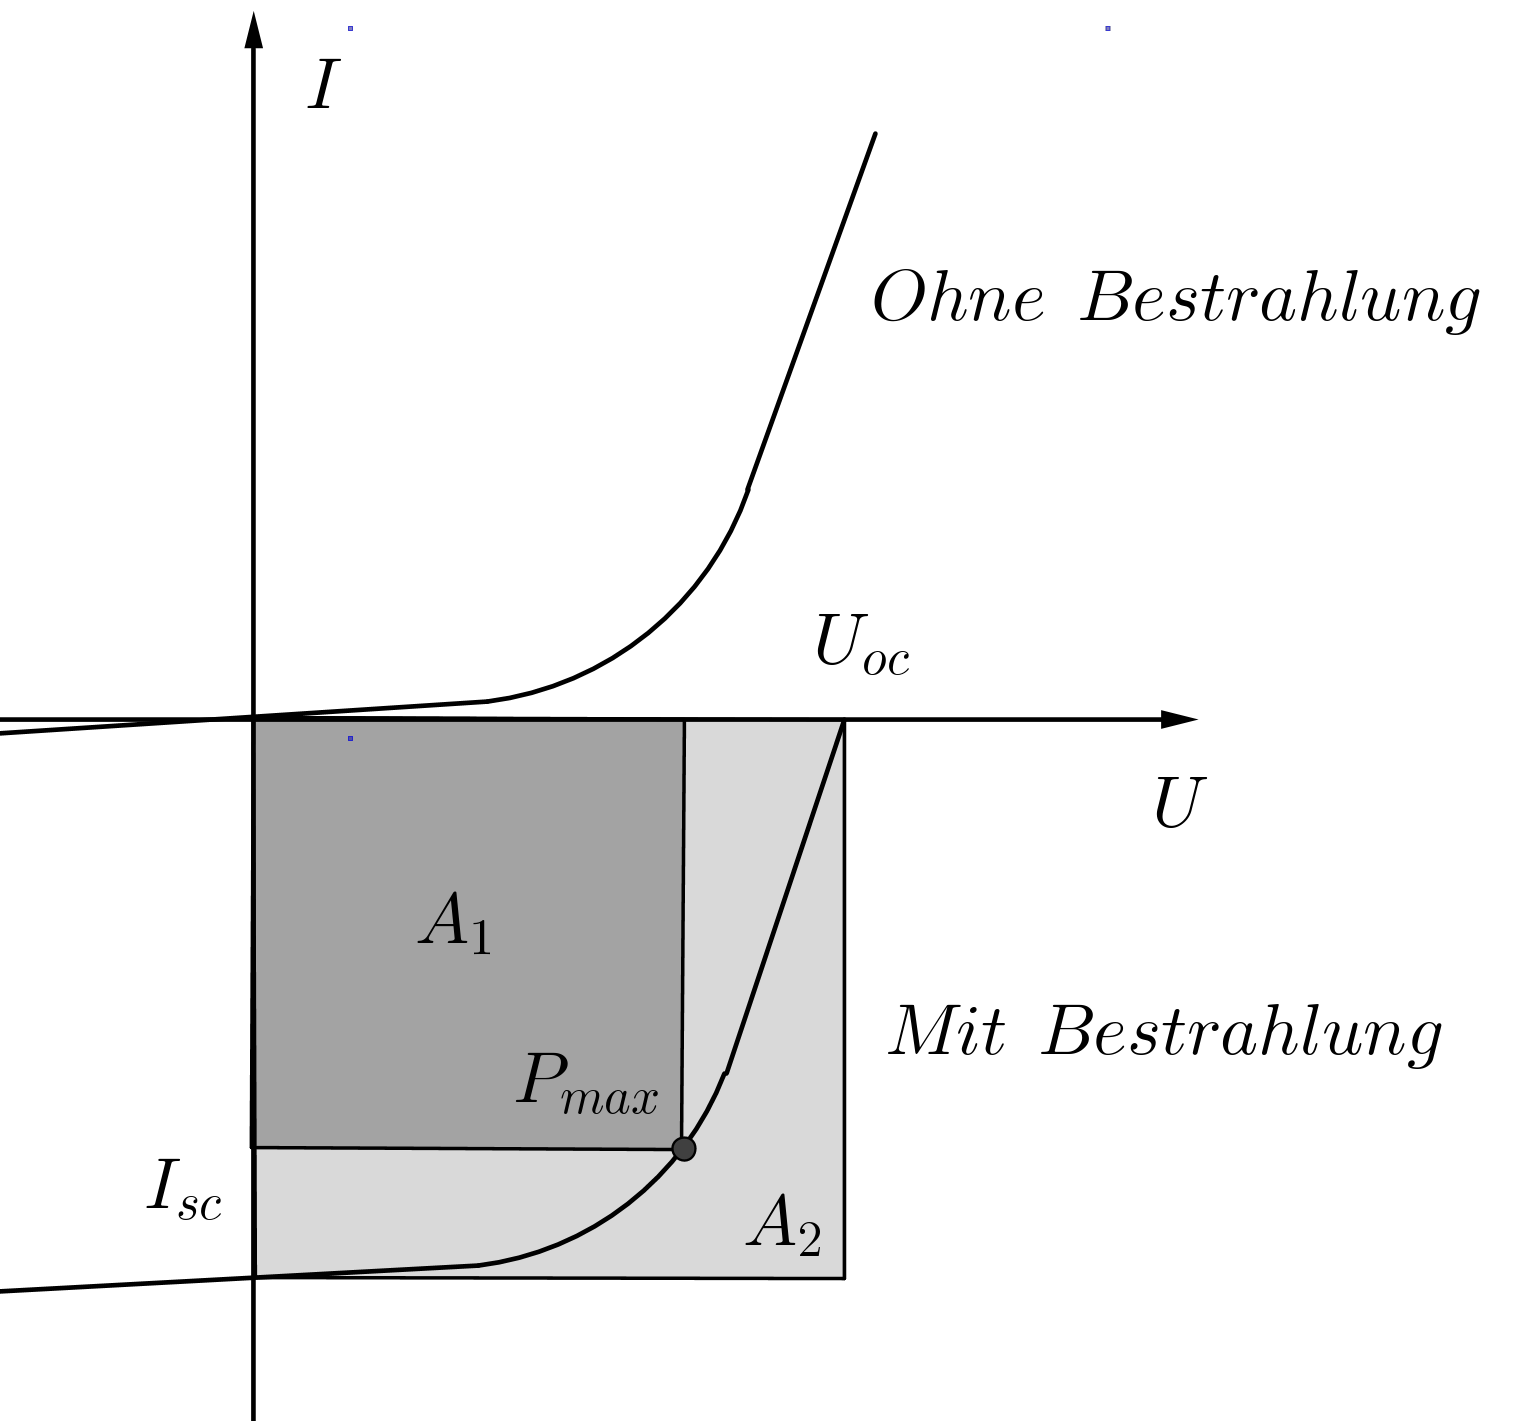
\includegraphics[width=0.5\textwidth]{pics/sol2.png}
\caption{Kennlinie einer Silizium-Solarzelle}
\label{Kennlinie}
\end{figure}

In Abbildung \ref{Kennlinie} schließt die Kennlinie an
diesem Punkt ein Rechteck A$_1$ ein, welches mit dem Rechteck A$_2$ einen Füllfaktor (FF = A$_1$ / A$_2$) ergibt. Der Wirkungsgrad $\eta$
setzt sich aus dem Verhältnis des maximalen Leistung und der eingestrahlten Leistung $P_{\text{ein}}$ zusammen.

\begin{equation}
 \eta = \frac{P_{\text{max}}}{P_{\text{ein}}} = \frac{U_{\text{oc}}\cdot I_{\text{sc}}\cdot \text{FF}}{P_{\text{ein}}}
\end{equation}

\section{Durchführung}
Ziel des Versuchs ist die Ermittlung der Strom-Spannungskennlinien einer Solarzelle für verschiedene Beleuchtungsstärken und daraus soll
die abgegebene Leistung der Solarzelle und deren Wirkungsgrad berechnet werden. Darüber hinaus sollen die Leerlaufspannung und der Kurzschlussstrom 
ebenfalls als Funktion der Beleuchtungsstärke bestimmt werden.\\
Hierzu wird die Solarzelle mit einer Lampe verstellbarer Höhe beleuchtet. Die Beleuchtungsstärke nimmt mit zunehmendem Abstand ab. 
Mit einem Volt- und einem Amperemeter werden die anliegende Spannung und der Strom für manuell einstellbare ohmsche Widerstände von 5 bis 300 $\Omega$ notiert. 

\section{Auswertung}
\subsection{Leerlaufspannung und Kurzschlussstrom}
Zunächst sollen die Leerlaufspannung und der Kurzschlussstrom der Solarzelle bestimmt werden. Hierfür wird die Widerstandsbrückenschaltung entfernt und die Solarzelle kurzgeschlossen.
Dann werden für verschiedene Abstände Messwerte aufgenommen.

\begin{figure}[H]
	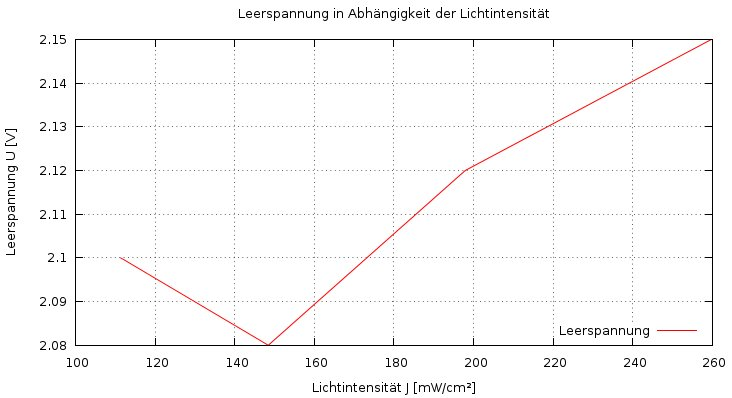
\includegraphics[width=\textwidth]{pics/Leerspannung_U.jpg}
	\caption{Leerspannung gegen Abstand zur Lichtquelle}
\end{figure}

Aus der Ausgleichsgeraden lässt sich der Proportionalitätsfaktor $a$ zwischen $I_K$ und $J$  errechnen zu
\begin{align*}
	a=0,291421 \pm 0,07142
\end{align*}

\begin{figure}[H]
	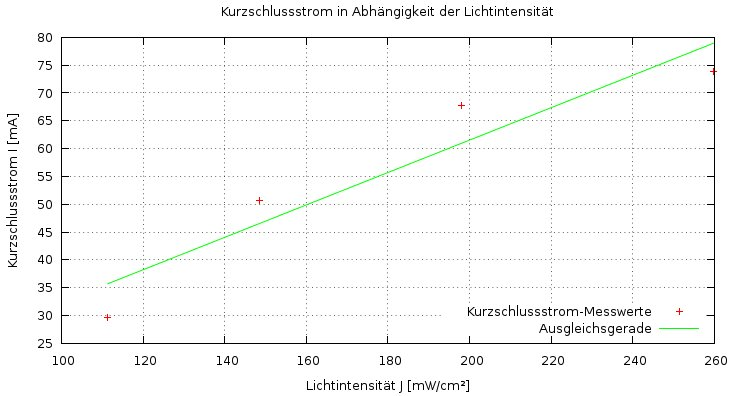
\includegraphics[width=1\textwidth]{pics/Kurzschluss_I_mit_gerade.jpg}
	\caption{Kurzschlussstrom gegen Abstand zur Lichtquelle mit Ausgleichsgerade}
\end{figure}

\subsection{U-I-Kennlinien}
Anschließend sollen die U-I-Kennlinien für vier verschiedene Abstände von der Lampe aufgenommen werden. Man misst dazu den Strom und die anliegende Spannung für verschiedene Widerstände und trägt beide gegeneinander auf. Zusätzlich stehen in den Tabellen die Leistung $P=U \cdot I$ in [mW] für spätere Auswertungen.


\renewcommand{\arraystretch}{0.83}
\begin{table}[H]
\begin{tabular}{|c|c|c|c|}
\hline 
Widerstand [$\Omega$]	&Strom [mA]	&Spannung [V]	&Leistung [mW]\\	
\hline
5	&27,8	&0,15	&4,2812\\
10	&27,9	&0,30	&8,2305\\
15	&27,7	&0,44	&12,1049\\
20	&27,8	&0,58	&16,1796\\
25	&27,7	&0,72	&19,8609\\
30	&27,4	&0,86	&23,4544\\
35	&27,4	&0,99	&27,0986\\
40	&27,3	&1,11	&30,3030\\
45	&27,0	&1,24	&33,4800\\
50	&26,7	&1,49	&39,7830\\
55	&26,3	&1,60	&42,0800\\
60	&25,5	&1,68	&42,8400\\
65	&24,8	&1,74	&43,1520\\
70	&23,9	&1,79	&42,7810\\
75	&22,9	&1,82	&41,6780\\
80	&22,0	&1,85	&40,7000\\
85	&21,0	&1,87	&39,2700\\
90	&20,1	&1,88	&37,7880\\
95	&19,2	&1,90	&36,4800\\
100	&18,5	&1,91	&35,3350\\
\hline 
\end{tabular}
\caption{Werte aufgenommen im Abstand von 70cm}
\end{table}
 
 \renewcommand{\arraystretch}{0,75}
 \begin{table}[H]
\begin{tabular}{|c|c|c|c|}
\hline 
Widerstand [$\Omega$]	&Strom [mA]	&Spannung [V]	&Leistung [mW]\\	
\hline
5	&48,7	&0,30	&14,6100\\
10	&48,5	&0,53	&25,7050\\
15	&48,7	&0,77	&37,4990\\
20	&48,7	&1,03	&50,1610\\
25	&48,5	&1,25	&60,6250\\
30	&48,2	&1,49	&71,8180\\
35	&46,3	&1,66	&76,8580\\
40	&43,2	&1,76	&76,0320\\
45	&39,8	&1,83	&72,8340\\
50	&36,8	&1,87	&68,8160\\
55	&33,9	&1,89	&64,0710\\
60	&31,4	&1,91	&59,9740\\
65	&29,2	&1,93	&56,3560\\
70	&27,4	&1,94	&53,1560\\
75	&25,7	&1,95	&50,1150\\
80	&24,2	&1,96	&47,4320\\
85	&22,9	&1,97	&45,1130\\
90	&21,7	&1,97	&42,7490\\
95	&20,6	&1,98	&40,7880\\
100	&19,7	&1,98	&39,0060\\
150	&13,4	&2,02	&27,0680\\
200	&10,1	&2,03	&20,5030\\
250	&8,1	&2,03	&16,4633\\
300	&6,7	&2,03	&13,6010\\
\hline 
\end{tabular}
\caption{Werte aufgenommen im Abstand von 60cm} 
\end{table}

\begin{table}[H]
\begin{tabular}{|c|c|c|c|}
\hline 
Widerstand [$\Omega$]	&Strom [mA]	&Spannung [V]	&Leistung [mW]\\	 
\hline 
5	&68,8	&0,38	&26,1440\\
10	&68,6	&0,73	&50,0780\\
15	&68,2	&1,00	&68,2000\\
20	&66,8	&1,38	&92,1840\\
25	&63,3	&1,63	&103,1790\\
30	&57,2	&1,76	&100,6720\\
35	&51,3	&1,83	&93,8790\\
40	&46,2	&1,87	&86,3940\\
45	&41,6	&1,90	&79,0400\\
50	&37,8	&1,92	&72,5760\\
55	&34,7	&1,93	&66,9710\\
60	&32,1	&1,95	&62,5950\\
65	&29,8	&1,96	&58,4080\\
70	&27,9	&1,97	&54,9630\\
75	&26,2	&1,98	&51,8760\\
80	&24,5	&1,98	&48,5100\\
85	&23,2	&1,99	&46,1680\\
90	&22,0	&1,99	&43,7800\\
95	&20,8	&1,99	&41,3920\\
100	&19,9	&1,99	&39,6010\\
150	&13,4	&2,02	&27,0680\\
200	&10,1	&2,03	&20,5030\\
300	&6,8	&2,05	&13,9400\\
\hline 
\end{tabular}
\caption{Werte aufgenommen im Abstand von 50cm}
\end{table}

\begin{table}[H]
\begin{tabular}{|c|c|c|c|}
\hline 
Widerstand [$\Omega$]	&Strom [mA]	&Spannung [V]	&Leistung [mW]\\	
\hline
5	&78,3	&0,46	&36,0180\\
10	&78,5	&0,84	&65,9400\\
15	&78,9	&1,23	&97,0470\\
20	&77,9	&1,61	&125,4190\\
25	&71,4	&1,83	&130,6620\\
30	&61,8	&1,90	&117,4200\\
35	&53,9	&1,92	&103,4880\\
40	&47,9	&1,95	&93,4050\\
45	&42,9	&1,96	&84,0840\\
50	&39,1	&1,98	&77,4180\\
55	&35,7	&1,99	&71,0430\\
60	&32,9	&2,00	&65,8000\\
65	&30,5	&2,01	&61,3050\\
70	&28,5	&2,01	&57,2850\\
75	&26,7	&2,02	&53,9340\\
80	&25,1	&2,02	&50,7020\\
85	&23,6	&2,03	&47,9080\\
90	&22,4	&2,03	&45,4720\\
95	&21,2	&2,03	&43,0360\\
100	&20,2	&2,03	&41,0060\\
150	&13,6	&2,05	&27,8800\\
200	&10,3	&2,06	&21,2180\\
250	&8,2	&2,07	&16,9740\\
300	&8,9	&2,07	&18,4230 \\
\hline 
\end{tabular}
\caption{Werte aufgenommen im Abstand von 40cm}
\end{table}
\renewcommand{\arraystretch}{1}

Gegeneinander aufgetragen ergeben diese Daten folgenden Graphen:

\begin{figure}[htbp]
	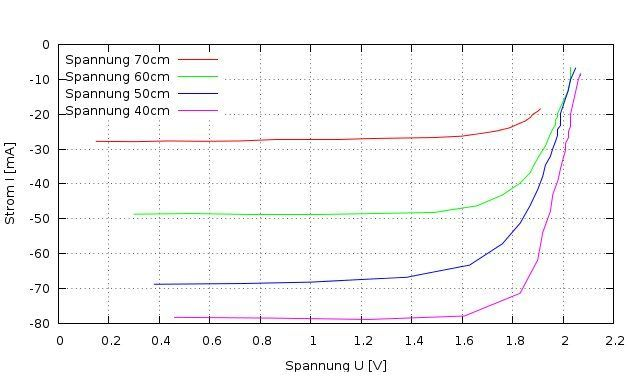
\includegraphics[width=\textwidth]{pics/alle_UI.jpg}
	\caption{U-I-Kennlinien für vier verschiedene Abstände}
\end{figure}

\subsection{Leistung}
Trägt man alle Leistungen gegen den Entsprechenden Schaltungswiderstand $\frac{U}{I}$ auf, so ergibt sich folgernder Graph:

\begin{figure}[H]
	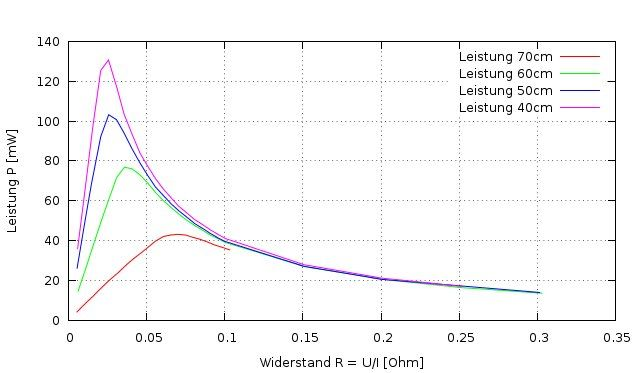
\includegraphics[width=0.75\textwidth]{pics/alle_L.jpg}
	\caption{Abgegebene Leistung in verschiedenen Abständen zur Strahlungsquelle}
\end{figure}

Die Leistung wird nicht gegen den Widerstand der Brückenschaltung aufgetragen, da sowohl das Amperemeter, als auch das Voltmeter noch einen nicht vernachlässigbaren Innenwiderstand haben.
Die Division von U und I liefert jedoch den korrekten Widerstand.

\subsection{Wirkungsgrad}
Die abgegebene Leistung ist abhängig vom Verhältnis zwischen der Spannung und dem Strom und weißt daher  ein Maximum auf. Dieses kann man bestimmen, indem man entweder das größtmöglichste Rechteck in den U-I-Graphen zeichnet, dessen Fläche entspricht der maximalen Ausgangsleistung der Solarzelle. Alternativ multipliziert man alle Spannungen mit den entsprechenden Strömen, trägt die Werte in einen Graphen ein und bestimmt den größten Wert. Da dies genauer ist, wurde die Leistung über diese Methode bestimmt.

Der Wirkungsgrad einer Solarzelle ist das Verhältnis zwischen der aufgenommenen Leistung (Licht) und der ausgegebenen Leistung (Elektrizität).
Die aufgenommene Leistung errechnet sich über eine kalibrierungskurve. In ihr wird die abgestrahlte Leistung der Lampe pro Fläche $[mW/cm^2]$ gegen den Abstand d dargestellt.\\

\begin{tabular}{|c|c|c|c|c|}
\hline 
Abstand & P pro $cm^2$ & $P_Eingang$ & $P_Gesamt$ & Wirkungsgrad $\eta$ \\ 
\hline 
70cm & 9mW & 445,48mW & 43,15mW & 0,0969 \\ 
\hline 
60cm & 12mW & 593,76mW & 76,86mW & 0,1242 \\ 
\hline 
50cm & 16mW & 791,68mW & 103,18mW & 0,1303 \\ 
\hline 
40cm  & 21mW & 1093,08mW & 130,66mW & 0,1258 \\ 
\hline 
\end{tabular} \\

Das Ausmessen der Solarzelle ergab eine Fläche von $49,48cm^2$. Durch Multiplikation dieses Wertes mit der abgestrahlten Leistung pro Fläche erhält man den Gesamtwert der aufgenommenen Leistung und aus Tabellen 1 bis 4 entnimmt man die maximale Gesamtausgangsleistung. Durch Division dieser beider Werte erhält man den Wirkungsgrad $\eta$ der Solarzelle. 
Gemittelt erhält man so
\begin{align*}
	\eta=0,1205 \pm 0,000253
\end{align*} 
Dieser Wert passt sehr gut mit den tatsächlichen Wirkungsgraden von polykristalinen Solarzellen überein, welche typischerweise Wirkungsgrade zwischen 14 und 20\% haben.
\section{Diskussion}
Die Ermittelung des Wirkungsgrades gelang mit den vorliegenden Daten hinreichend genau. 
Aus den Graphen kann man eine nicht-lineare Abhängigkeit zwischen Ausgangsleistung und Abstand zur Lichtquelle ablesen, welcher auf Grund des Raumwinkels proportional zu $\frac{1}{R^2}$ sein müsste.\\
Die Leerlaufspannung bleibt unabhängig von der Lichtintensität relativ konstant zwischen 2,08 und 2,15V. Da sie nur beim zweiten Messpunkt nach unten abweicht, kann davon ausgegangen werden, dass es sich dabei um einen Messfehler handelt. In Anbetracht der Größe der Abweichung kann desweiteren davon ausgegangen werden, dass auch die anderen Werte ähnlichen Schwankungen unterliegen und die Leerspannung eigentlich immer konstant sein müsste. Aus Diagramm 4 lässt sich dies noch besser ablesen, da alle Kurven zwar bei unterschiedlichen Y-Achsen-Werten starten, jedoch alle die X-Achse beim etwa gleichen Wert durchstoßen.  Genauere Klärung würden hier mehr Messreihern geben, die leider nicht vorliegen.\\
Abschließend stellt sich die Frage, in wie weit ein Wirkungsgrad dieser Größenordnung gegen die Wirtschaftlichkeit der Verwendung von Solarzellen zur Stromerzeugung spricht. Insbesonden in Deutschland ist die Sonneneinstrahlung nicht sehr hoch und die Zeiten, in denen der Himmel nicht wolkenverhangen ist, sind so kurz, dass es sich nicht rentiert, wenn jeder Bürger Solarzellen auf seinem Dach montiert.
Betrachtet man zudem die hohen Herstellungskosten, die verhältnismäßig geringe Lebensdauer trotz ständiger Wartung und der Energieverbrauch bei der Herstellung, so scheinen Solarzellen nicht die Lösung für das Weltenergieproblem zu sein. Man muss Standortbezogen entscheiden, welche regenerativen Energien die meiste Energie liefern und dann den Strom durch einen Zusammenschluss aller Energien erzeugen, um nachhaltig Elektrizität in benötigter Menge zu erzeugen. 
% ========================================
%	Literaturverzeichnis
% ========================================

%\bibliographystyle{plainnat}			% Bibliographie-Style auswählen
%\bibliography{BIBDATEI}			% Literaturverzeichnis

% ========================================
%	Das Dokument endent
% ========================================

\end{document}
